\begin{wrapfigure}{r}{0.25\textwidth}
\caption{Схема к задаче с демпингом пружинки}\label{wrap-fig:3}
\centering
\tikzset{every picture/.style={line width=0.75pt}} %set default line width to 0.75pt        

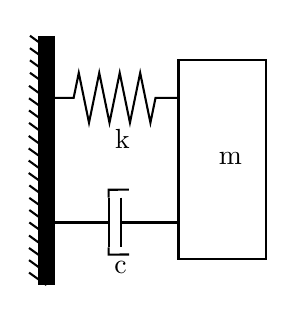
\begin{tikzpicture}[x=0.75pt,y=0.75pt,yscale=-0.6,xscale=0.6]
%uncomment if require: \path (0,300); %set diagram left start at 0, and has height of 300

%Straight Lines [id:da4887670776446218] 
\draw [line width=6]    (184,0) -- (184,200) ;
%Straight Lines [id:da28801859217306736] 
\draw    (170,190) -- (184,200) ;
%Straight Lines [id:da1637896396436871] 
\draw    (170,180) -- (183.75,190) ;
%Straight Lines [id:da62875004275454] 
\draw    (170,170.25) -- (184,180.25) ;
%Straight Lines [id:da6006085071609413] 
\draw    (170,160.25) -- (183.75,170.25) ;
%Straight Lines [id:da05691598933749353] 
\draw    (170.25,149.75) -- (184.25,159.75) ;
%Straight Lines [id:da9579907895748434] 
\draw    (170.25,139.75) -- (184,149.75) ;
%Straight Lines [id:da3248601744537396] 
\draw    (170.25,130) -- (184.25,140) ;
%Straight Lines [id:da2179948770685416] 
\draw    (170.25,120) -- (184,130) ;
%Straight Lines [id:da010333354574830755] 
\draw    (169.75,110.05) -- (183.75,120.05) ;
%Straight Lines [id:da8360274619825747] 
\draw    (169.75,100.05) -- (183.5,110.05) ;
%Straight Lines [id:da5215109964501989] 
\draw    (169.75,90.3) -- (183.75,100.3) ;
%Straight Lines [id:da324252128845288] 
\draw    (169.75,80.3) -- (183.5,90.3) ;
%Straight Lines [id:da4166166100945381] 
\draw    (170,59.8) -- (183.75,69.8) ;
%Straight Lines [id:da15015174115931007] 
\draw    (170,50.05) -- (184,60.05) ;
%Straight Lines [id:da8895760399397958] 
\draw    (170,40.05) -- (183.75,50.05) ;
%Straight Lines [id:da5966438059287478] 
\draw    (170.75,29.55) -- (184.75,39.55) ;
%Straight Lines [id:da6544673898899798] 
\draw    (170.75,19.55) -- (184.5,29.55) ;
%Straight Lines [id:da9924453204265613] 
\draw    (170.75,9.8) -- (184.75,19.8) ;
%Straight Lines [id:da6315114461783526] 
\draw    (170.75,-0.2) -- (184.5,9.8) ;
%Shape: Resistor [id:dp9867652168405341] 
\draw   (187.35,49.65) -- (205.84,49.65) -- (209.95,29.65) -- (218.17,69.65) -- (226.39,29.65) -- (234.61,69.65) -- (242.82,29.65) -- (251.04,69.65) -- (259.26,29.65) -- (267.48,69.65) -- (271.59,49.65) -- (290.08,49.65) ;
%Straight Lines [id:da4443636395724011] 
\draw    (170,69.8) -- (183.75,79.8) ;
%Shape: Capacitor [id:dp782467290213184] 
\draw   (188,149.8) -- (233.94,149.8) (244.14,129.8) -- (244.14,169.8) (233.94,129.8) -- (233.94,169.8) (244.14,149.8) -- (290.08,149.8) ;
%Shape: Right Angle [id:dp6966591703655525] 
\draw   (233.94,129.8) -- (233.89,123.5) -- (250.25,123.38) ;
%Shape: Right Angle [id:dp6346918568418609] 
\draw   (233.94,169.8) -- (233.98,175.57) -- (250.34,175.44) ;
%Shape: Rectangle [id:dp21808439716841233] 
\draw   (290,19.33) -- (360,19.33) -- (360,179.33) -- (290,179.33) -- cycle ;

% Text Node
\draw (236.61,72.65) node [anchor=north west][inner sep=0.75pt]   [align=left] {k};
% Text Node
\draw (320,91.33) node [anchor=north west][inner sep=0.75pt]   [align=left] {m};
% Text Node
\draw (235.98,178.57) node [anchor=north west][inner sep=0.75pt]   [align=left] {c};


\end{tikzpicture}
\end{wrapfigure}